\documentclass{article}

\usepackage{graphicx}
\usepackage{tikz}
\usepackage{tikzsymbols}
\usetikzlibrary{calc,patterns,shapes.geometric}
\pagestyle{empty}
\usepackage[margin=0pt]{geometry}
\geometry{papersize={14in,12in}}

\def\centerarc[#1](#2)(#3:#4:#5){\draw[#1] ($(#2)+({#5*cos(#3)},{#5*sin(#3)})$) arc (#3:#4:#5);}

\begin{document}
	\begin{figure}
		\centering
		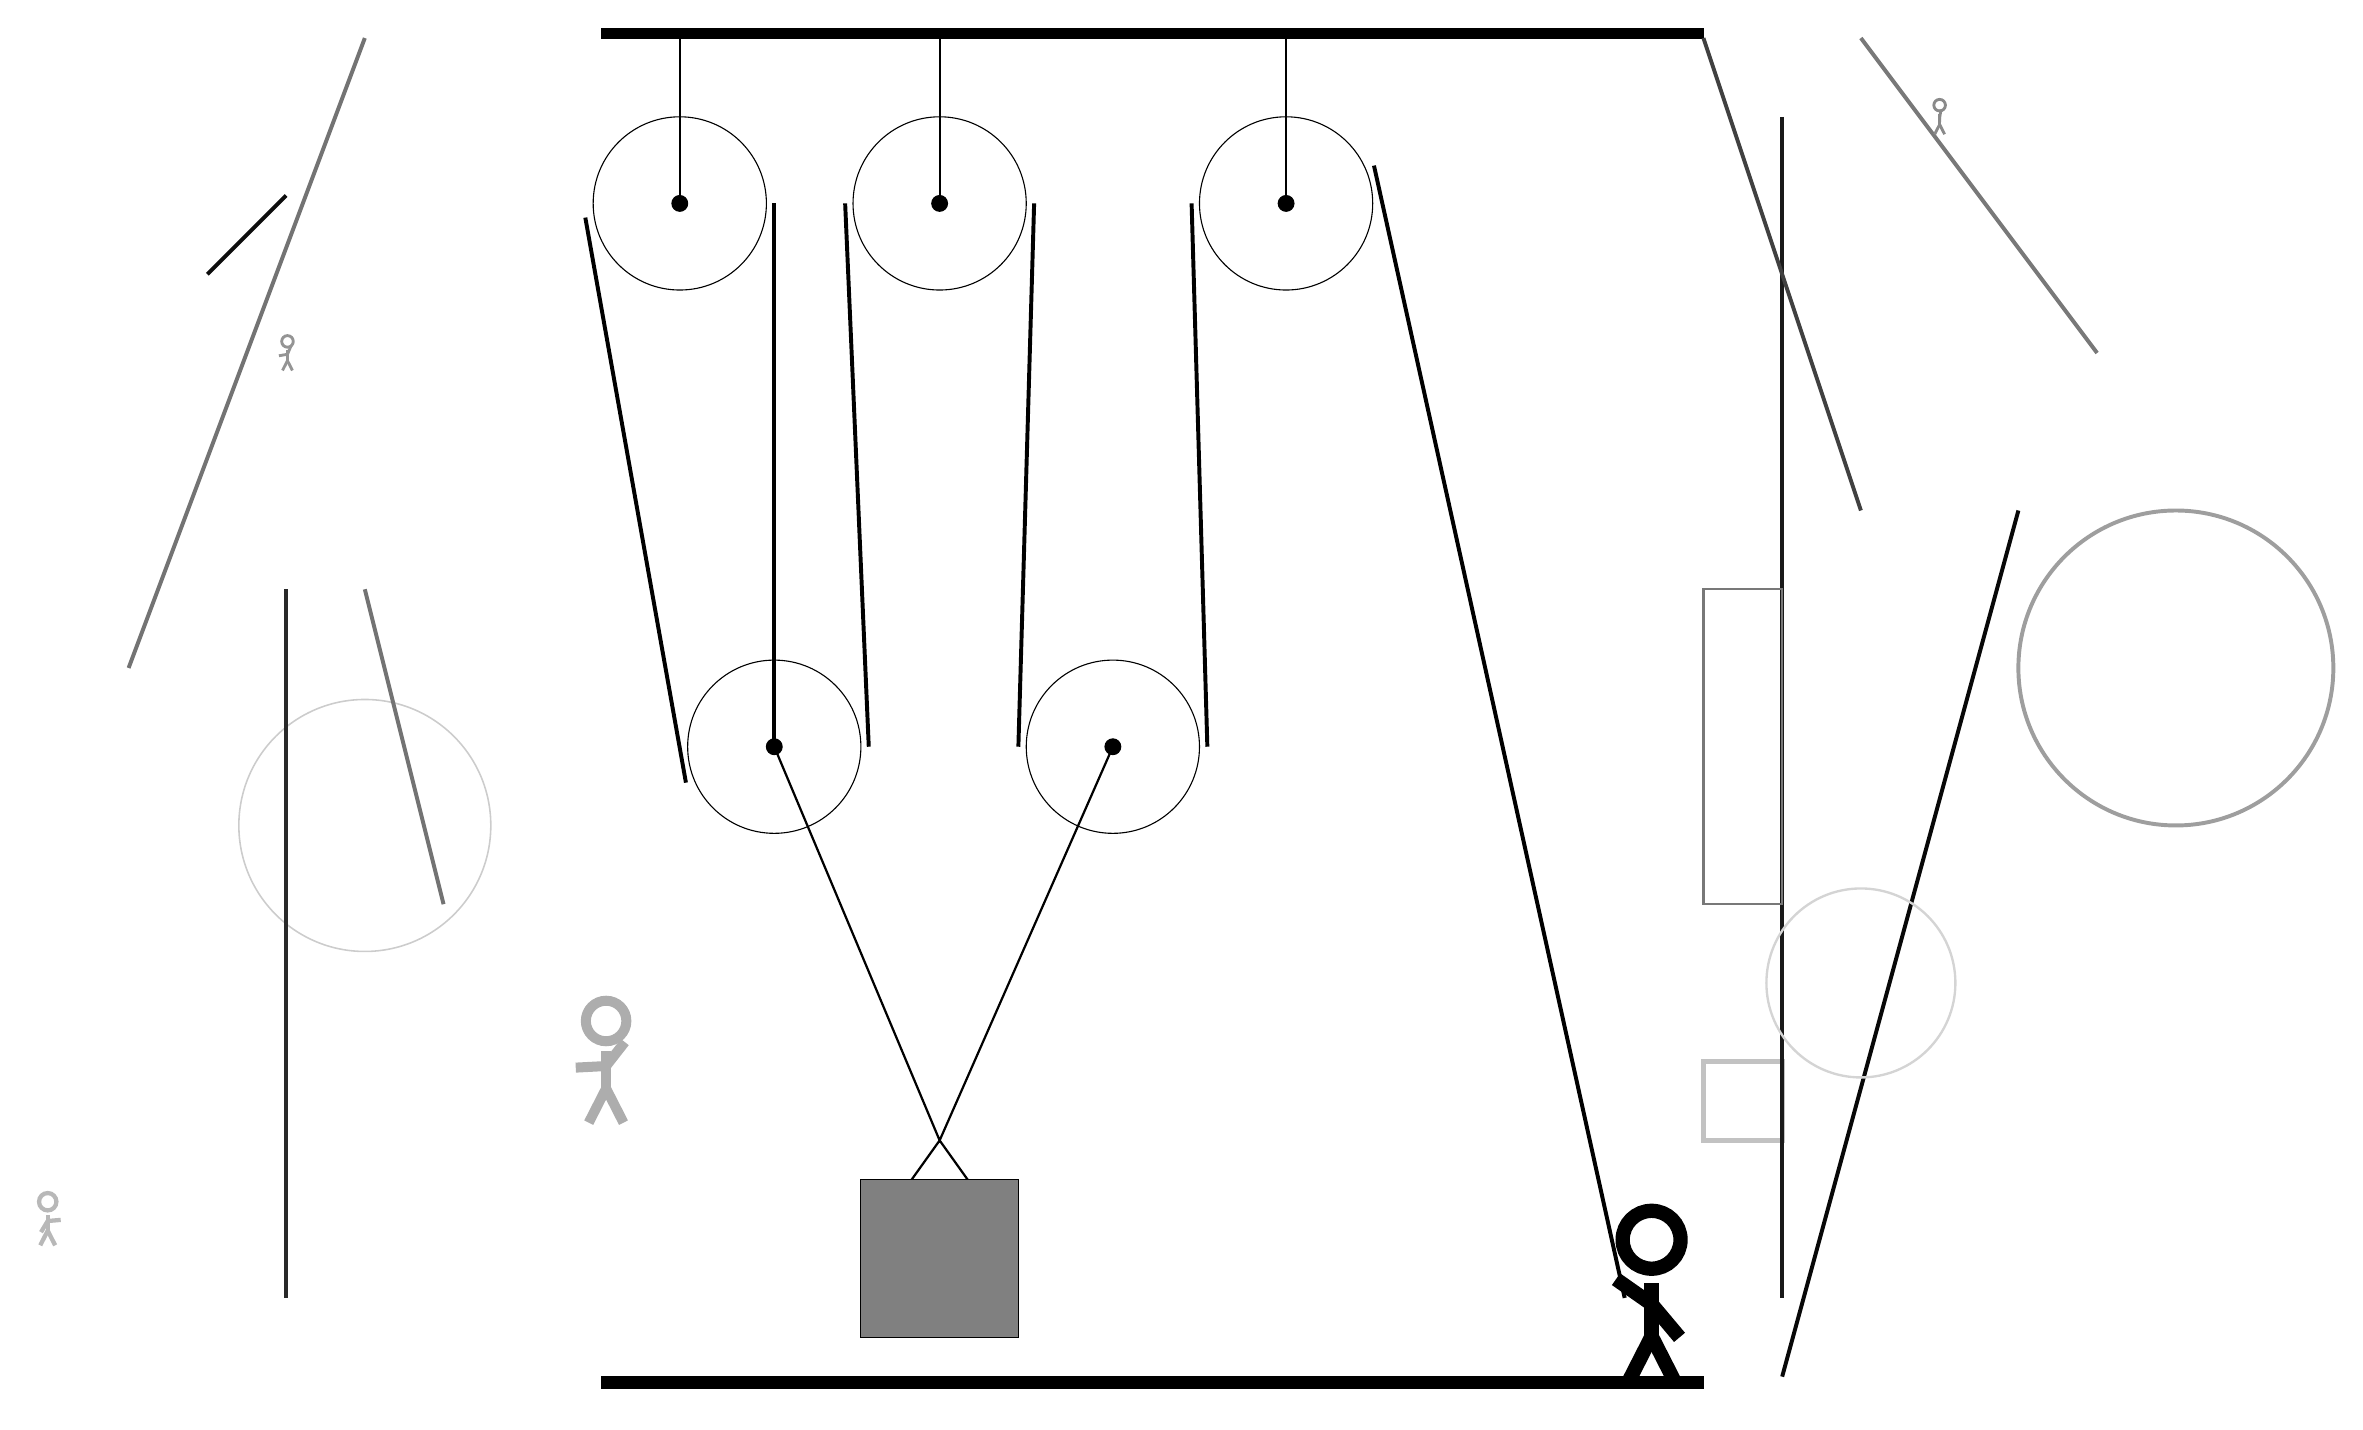
\begin{tikzpicture}
			%%%%% START %%%%%
			
			\draw[fill=black] (-2, 14) rectangle (12, 14.125);
			
			\draw (-1, 11.9) circle (1.1);
			\draw[fill=black] (-1, 11.9) circle (0.1);
			\draw[thick] (-1, 11.9) -- (-1, 14);
			
			\draw [line width=0.2mm, color=black!20](-5, 4) circle (1.6);
			
			\node[line width=0.3mm, color=black!42] at (-6, 10) {\Strichmaxerl[2][10][67]};
			\draw[line width=0.5mm, color=black!97](16, 8) -- (13, -3);
			\draw[line width=0.6mm, color=black!24] (13, 1) rectangle (12, 0);
			\draw[line width=0.5mm, color=black!53](14, 14) -- (17, 10);
			
			\draw[line width=0.5mm, color=black!55](-4, 3) -- (-5, 7);
			\draw[line width=0.5mm, color=black!90](13, 13) -- (13, -2);
			\draw[line width=0.5mm, color=black!75](12, 14) -- (14, 8);
			\draw[line width=0.5mm, color=black!84](-6, -2) -- (-6, 7);
			\draw[line width=0.5mm, color=black!95](-7, 11) -- (-6, 12);
			\node[line width=0.5mm, color=black!32] at (-2, 1) {\Strichmaxerl[7][3][52]};
			
			\draw[line width=0.5mm, color=black!55](-5, 14) -- (-8, 6);
			\draw[line width=0.3mm, color=black!53] (12, 3) rectangle (13, 7);
			
			\draw [line width=0.5mm, color=black!38](18, 6) circle (2.0);
			\node[line width=0.4mm, color=black!46] at (15, 13) {\Strichmaxerl[2][89][81]};
			\node[line width=0.7mm, color=black!28] at (-9, -1) {\Strichmaxerl[3][59][5]};
			
			\draw [line width=0.3mm, color=black!17](14, 2) circle (1.2);
			
			\draw (2.3, 11.9) circle (1.1);
			\draw[fill=black] (2.3, 11.9) circle (0.1);
			\draw[thick] (2.3, 11.9) -- (2.3, 14);
			
			\draw (6.7, 11.9) circle (1.1);
			\draw[fill=black] (6.7, 11.9) circle (0.1);
			\draw[thick] (6.7, 11.9) -- (6.7, 14);
			
			\draw (0.2, 5) circle (1.1);
			\draw[fill=black] (0.2, 5) circle (0.1);
			
			\draw (4.5, 5) circle (1.1);
			\draw[fill=black] (4.5, 5) circle (0.1);
			
			\draw[thick] (0.2, 5) -- (2.3, 0)  -- (4.5, 5);
			\draw[thick]  (1.8, -0.7) -- (2.3, 0) -- (2.8, -0.7);
			\draw[fill=black!50] (1.3, -0.5) rectangle (3.3, -2.5);
			
			\draw[line width=0.5mm] (0.2, 5) -- (0.2, 11.9);
			\centerarc[line width=0.5mm](-1, 11.9)(0:200:1.2000000000000002);
			\draw[line width=0.5mm] (-2.2, 11.72) -- (-0.922, 4.544);
			\centerarc[line width=0.5mm](0.2, 5)(200:360:1.2000000000000002);
			\draw[line width=0.5mm](1.4, 5) -- (1.1, 11.9);
			\centerarc[line width=0.5mm](2.3, 11.9)(0:180:1.2000000000000002);
			\draw[line width=0.5mm] (3.5, 11.9) -- (3.3, 5);
			\centerarc[line width=0.5mm](4.5, 5)(180:360:1.2000000000000002);
			\draw[line width=0.5mm] (5.7, 5) -- (5.5, 11.9);
			\centerarc[line width=0.5mm](6.7, 11.9)(20:180:1.2000000000000002);
			\draw[line width=0.5mm](7.816, 12.38)  -- (11, -2);
			
			\node at (11.3, -2) {\Strichmaxerl[10][-35][-50]};
			
			\draw[fill=black] (-2, -3) rectangle (12, -3.15);
			
			%%%%% END %%%%%
		\end{tikzpicture}
	\end{figure}	
\end{document}